\documentclass[11pt]{article}
\usepackage[margin=1.1in]{geometry}
\usepackage{amsmath,amssymb,amsthm}
\usepackage{booktabs}
\usepackage{microtype}
\usepackage{xcolor}
\usepackage{tikz}
\usetikzlibrary{positioning,arrows.meta,calc,fit,backgrounds,shapes.geometric,decorations.pathreplacing}
\usepackage[colorlinks=true,linkcolor=blue!50!black,citecolor=blue!50!black,urlcolor=blue!50!black]{hyperref}
\emergencystretch=2em
% float placement: this paper is figure-dense; let them settle near their text
\setcounter{topnumber}{3}
\setcounter{bottomnumber}{2}
\setcounter{totalnumber}{5}
\renewcommand{\topfraction}{0.9}
\renewcommand{\bottomfraction}{0.7}
\renewcommand{\textfraction}{0.07}
\renewcommand{\floatpagefraction}{0.7}
\newcommand{\code}[1]{\texttt{#1}}
\newtheorem{theorem}{Theorem}
\newtheorem{principle}{Principle}

% ---- figure visual language: proved = solid, learned = dashed ----
\definecolor{provedc}{RGB}{31,84,140}
\definecolor{learnedc}{RGB}{176,94,20}
\definecolor{datac}{RGB}{90,90,90}
\tikzset{
  proved/.style   = {draw=provedc, very thick, fill=provedc!6, rounded corners=2pt,
                     align=center, inner sep=4pt, font=\small},
  learned/.style  = {draw=learnedc, very thick, dashed, fill=learnedc!6, rounded corners=2pt,
                     align=center, inner sep=4pt, font=\small},
  datum/.style    = {draw=datac, thick, fill=datac!5, rounded corners=2pt,
                     align=center, inner sep=4pt, font=\small},
  waist/.style    = {draw=provedc, very thick, fill=provedc!16, rounded corners=3pt,
                     align=center, inner sep=5pt, font=\small\bfseries},
  bad/.style      = {draw=red!65!black, very thick, dotted, fill=red!5, rounded corners=2pt,
                     align=center, inner sep=4pt, font=\small},
  flow/.style     = {-{Stealth[length=2.4mm]}, thick, draw=datac!140},
  thm/.style      = {font=\scriptsize\itshape, text=provedc, align=center},
  lbl/.style      = {font=\scriptsize, text=datac!150, align=center},
}

\title{GSLT2GSLT: Typed Action Decoding over Verified Interfaces\\
\large A machine-checked waist for neural program synthesis, and the belief-state
architecture it licenses}
\author{Oru\v{z}i \and Zarathustra Goertzel}
\date{July 2026 --- working draft}

\begin{document}
\maketitle

\begin{abstract}
We describe an architecture for neural program synthesis over generalized
syntax--semantics language theories (GSLTs) in which the interface between learning and
logic is machine-checked. The network never emits program text: it scores \emph{typed
construction actions} over an exact elaboration state, and a checker owns legality,
completion, and acceptance. Three layers are formalized in Lean~4 with kernel-checked
proofs: the discrete skeleton (legality masks proved sound, complete, and free of dead
ends), a \emph{trust boundary} (learned signals may reorder search but provably cannot
lose solutions; hard pruning is licensed exactly by per-property recall certificates,
with a machine-checked counterexample showing a plausible uncertified mask destroying a
genuine solution), and a \emph{decoder-state theory} (recurrent workspaces as damped
fixed-point iteration, with a finite optimal settling depth, a parallel-scan correctness
license, and a belief-state cell whose fusion rule is Bayesian conditioning). A single
lemma family shows Kalman updating, gated recurrent mixing, and probabilistic-logic
evidence revision to be one operation---addition of evidence in natural coordinates,
seen from the moment chart. Empirically, the resulting typed-action decoder replicates
Alien-Coding-style cumulative self-improvement on OEIS program discovery, with every
increment exactly verified; a twelve-cell factorial disentangles decoder architecture
from auxiliary supervision; and the same interface, pointed at an external dependent-type
benchmark, \emph{measured} the benchmark's definitional-equality demands
($\beta\eta$) through a graded ladder of verified roots. We state the open comparison
the theory sharpens: whether building Bayesian fusion into the decoder beats learning
Bayes-shaped mixing, and where---by theorem---learning is necessary because the world
does not hold still.
\end{abstract}

\section{Introduction}
\label{sec:intro}

Neural program synthesis systems typically trust a language model to emit well-formed
programs and filter failures afterwards. We invert the trust: the target language---a
GSLT, given as data---induces an exact elaboration state with typed holes; the network
only \emph{ranks legal refinements}; the checker computes what each refinement entails
and decides acceptance. The scientific benefit is attributability. When the interface
between proposer and checker is itself proved correct, a discovery cannot be an artifact
of a malformed candidate, and a failure cannot hide an interface bug: three times in the
development reported here, an apparent neural failure was traced by the formal layer to
an interface boundary (a mask dead-end, a defaulted intermediate type, a missing
conversion rule) \emph{before} any training run could mis-attribute it to learning.

The architecture is a waist (Figure~\ref{fig:waist}): one small action vocabulary through
which all learning speaks. Everything above the waist (encoders, decoder state, ranking,
search order) is free; everything below it (legality, spine construction, acceptance) is
checked; and the boundary itself is a pair of theorems rather than a convention.

\begin{figure}[htbp]
\centering
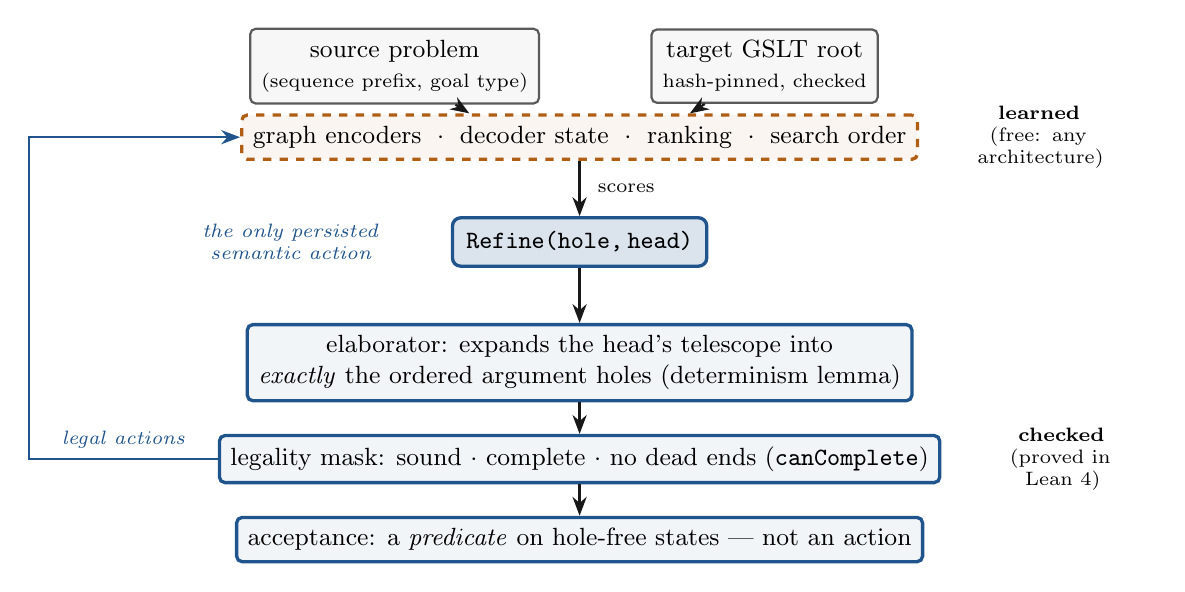
\begin{tikzpicture}[node distance=5mm]

% --- learned half -------------------------------------------------------
\node[datum] (src) {source problem\\{\scriptsize(sequence prefix, goal type)}};
\node[datum, right=14mm of src] (root) {target GSLT root\\{\scriptsize hash-pinned, checked}};
\node[learned, below=6mm of $(src)!0.5!(root)$, minimum width=62mm] (enc)
  {graph encoders \;$\cdot$\; decoder state \;$\cdot$\; ranking \;$\cdot$\; search order};
\node[lbl, right=3mm of enc, text width=22mm] {\textbf{learned}\\(free: any\\architecture)};

% --- the waist ----------------------------------------------------------
\node[waist, below=7mm of enc] (waist) {\code{Refine(hole,\,head)}};
\node[thm, left=4mm of waist, text width=30mm] {the only persisted\\semantic action};

% --- checked half -------------------------------------------------------
\node[proved, below=7mm of waist, minimum width=62mm] (elab)
  {elaborator: expands the head's telescope into\\
   \emph{exactly} the ordered argument holes (determinism lemma)};
\node[proved, below=4mm of elab, minimum width=62mm] (mask)
  {legality mask: sound $\cdot$ complete $\cdot$ no dead ends (\code{canComplete})};
\node[proved, below=4mm of mask, minimum width=62mm] (acc)
  {acceptance: a \emph{predicate} on hole-free states --- not an action};
\node[lbl, right=3mm of mask, text width=22mm] {\textbf{checked}\\(proved in\\Lean~4)};

% --- flows --------------------------------------------------------------
\draw[flow] (src) -- ($(enc.north)+(-14mm,0)$);
\draw[flow] (root) -- ($(enc.north)+(14mm,0)$);
\draw[flow] (enc) -- node[lbl,right=1mm] {scores} (waist);
\draw[flow] (waist) -- (elab);
\draw[flow] (elab) -- (mask);
\draw[flow] (mask) -- (acc);
% feedback: legal action set back up to the policy
\draw[flow, provedc] ($(mask.west)+(0,0)$) -- ++(-24mm,0)
  node[thm, midway, above] {legal actions}
  |- (enc.west);

\end{tikzpicture}
\caption{The waist. All learning speaks through one action vocabulary; the checker owns
what each action entails and whether a state is accepted. The narrow interface is what
makes architecture comparisons attributable: nothing above the waist can widen what is
acceptable below it.}
\label{fig:waist}
\end{figure}

\section{The waist: \code{Refine(hole, head)}}
\label{sec:waist}

The persisted semantic action is the pair \emph{refine this typed hole with this head}.
Dependent argument holes are not actions: applying a head expands, deterministically,
into exactly the ordered argument holes its telescope dictates (a determinism lemma,
not a convention). Termination is not an action: acceptance is a predicate on states
with no open holes. A policy may factor its score as
$P(\text{hole}\mid s)\,P(\text{head}\mid s,\text{hole})$, but the interface persists
the pair.

For the first-order root (a 16-operator combinator DSL for integer-sequence programs,
after \cite{gauthier2023}), the legality automaton is specified and sealed in Lean:
soundness (accepted streams parse to well-formed programs), completeness (every
well-formed program within budget is reachable with every prefix legal), and
\emph{no dead ends}---from every reachable legal state some completion exists within
budget (\code{canComplete}). The completion relation is exported with provenance: the
operator table and mask fixtures that the Python trainer consumes are generated from
the Lean development and hash-pinned, so the learned system and the proved system share
one source of truth. The same atomic interface is then instantiated for a dependent
typed-hole root (Section~\ref{sec:ladder-out}), with a proved equivalence to the sealed
first-order automaton as the non-vacuity gate: if the generic interface could not
express the sealed machine exactly, the interface would be wrong.

\section{The trust boundary}
\label{sec:trust}

Two theorems, proved once over the root-parametric interface, fix what learned signals
may do.

\begin{theorem}[Soft ranking is always safe]
Any external ranking that lists exactly the legal actions---in any order, from any
scorer, at any parameters---preserves the accepted language. Learned guidance can
reorder search; it cannot lose or manufacture solutions.
\end{theorem}

\begin{theorem}[Hard pruning is licensed exactly by certificates]
A pruning mask derived from a property \emph{certified for the target under the
evaluation semantics} never prunes a state from which a target-reproducing completion
exists (\code{certifiedMask\_recall\_preserving}, lifted from completed programs to
partial search states). Sign, parity, and modular-residue certificates instantiate the
schema.
\end{theorem}

The pair is kept honest by a mandatory counterexample: a plausible, uncertified
parity-of-root mask is exhibited, machine-checked, pruning the genuine constant-one
solution (\code{oddRootHardMask\_prunes\_oneSolution}). Uncertified evidence---including
everything a world model merely \emph{believes}---receives soft authority only; a
world-model hook converts a certified proposition into a licensed mask, and an empty
evidence slot fails the premise. This is the design doctrine ``the model proposes, the
checker disposes'' upgraded to mathematics, with the failure mode it prevents exhibited
rather than asserted. Figure~\ref{fig:trust} is the whole boundary on one page.

\begin{figure}[htbp]
\centering
\resizebox{\textwidth}{!}{%
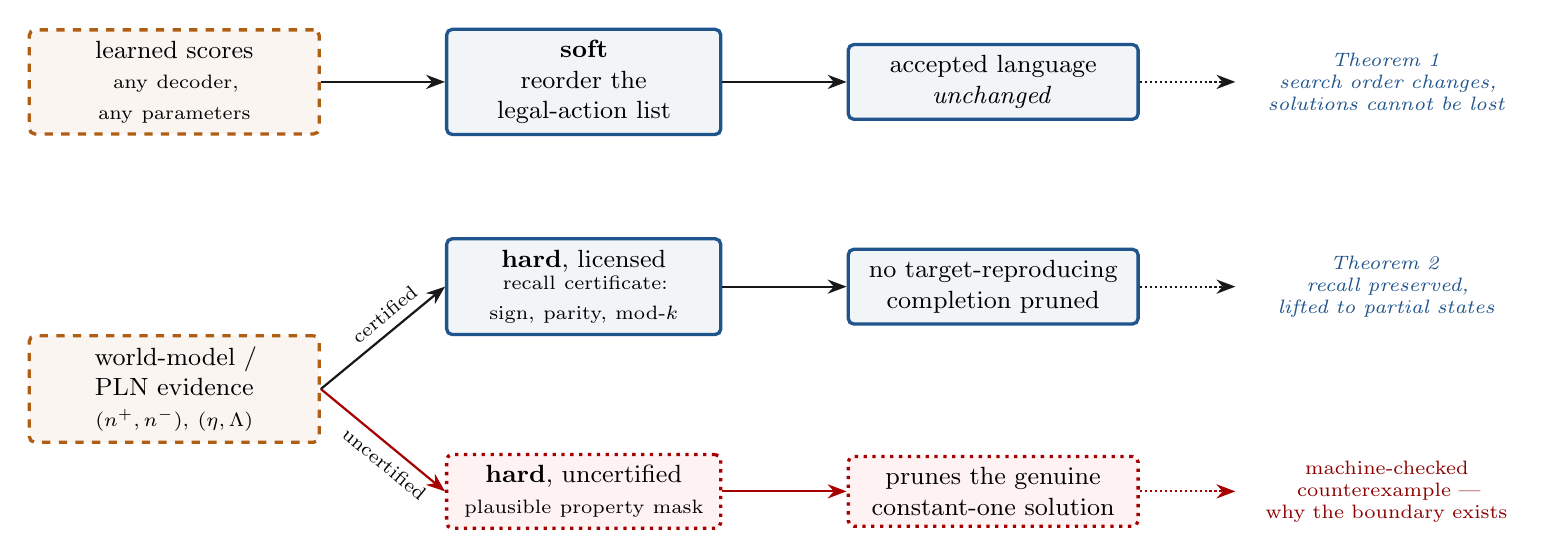
\begin{tikzpicture}

% three rows, explicit coordinates: y = 0 (soft), -26 (certified hard), -52 (uncertified hard)
\node[learned, text width=34mm] (score) at (0,0)
  {learned scores\\{\scriptsize any decoder, any parameters}};
\node[learned, text width=34mm] (wm) at (0,-39mm)
  {world-model / PLN evidence\\{\scriptsize$(n^{+},n^{-})$, $(\eta,\Lambda)$}};

\node[proved, text width=32mm] (soft) at (52mm,0)
  {\textbf{soft}\\reorder the legal-action list};
\node[proved, text width=32mm] (cert) at (52mm,-26mm)
  {\textbf{hard}, licensed\\{\scriptsize recall certificate:\\sign, parity, mod-$k$}};
\node[bad, text width=32mm] (unc) at (52mm,-52mm)
  {\textbf{hard}, uncertified\\{\scriptsize plausible property mask}};

\node[proved, text width=34mm] (safe1) at (104mm,0)
  {accepted language\\\emph{unchanged}};
\node[proved, text width=34mm] (safe2) at (104mm,-26mm)
  {no target-reproducing\\completion pruned};
\node[bad, text width=34mm] (fail) at (104mm,-52mm)
  {prunes the genuine\\constant-one solution};

\node[thm, text width=36mm] (t1) at (154mm,0) {Theorem~1\\search order changes,\\solutions cannot be lost};
\node[thm, text width=36mm] (t2) at (154mm,-26mm) {Theorem~2\\recall preserved,\\lifted to partial states};
\node[lbl, text width=36mm, text=red!55!black] (t3) at (154mm,-52mm)
  {machine-checked\\counterexample ---\\why the boundary exists};

\draw[flow] (score) -- (soft);
\draw[flow] (wm.east) -- node[lbl, above, sloped, pos=0.6] {certified} (cert.west);
\draw[flow, red!65!black] (wm.east) -- node[lbl, below, sloped, pos=0.6] {uncertified} (unc.west);
\draw[flow] (soft) -- (safe1);
\draw[flow] (cert) -- (safe2);
\draw[flow, red!65!black] (unc) -- (fail);
\draw[flow, densely dotted] (safe1) -- (t1.west);
\draw[flow, densely dotted] (safe2) -- (t2.west);
\draw[flow, densely dotted, red!65!black] (fail) -- (t3.west);

\end{tikzpicture}}
\caption{The trust boundary. Learned signals may always reorder; they may exclude only
behind a certificate. The red branch is not a caution but a theorem: a plausible
uncertified mask provably destroys a real solution.}
\label{fig:trust}
\end{figure}

\section{Decoder state: from one gated vector to a belief workspace}
\label{sec:state}

The incumbent decoder carries construction history in a single gated recurrent vector.
Its natural generalization is a \emph{workspace}: slots with fixed addresses and
evolving contents, updated by reusable read--transform--gate--write operators
\begin{equation}
w_i \;\leftarrow\; w_i + \tfrac{1}{K}\sum_{k=1}^{K} g_{ki}\,(c_{ki}-w_i),
\label{eq:workspace}
\end{equation}
an architecture family we adapt from an unpublished recurrent-workspace design
(personal communication, 2026), itself descended from external-memory networks and
shared-workspace models \cite{goyal2021}. Our adaptation types the addresses: slots are
indexed by the typed holes of the elaboration state, so the workspace is a typed
register file on which the program graph grows, and slot allocation is total and
injective by the sealed open-hole bound.

\begin{figure}[htbp]
\centering
\resizebox{\textwidth}{!}{%
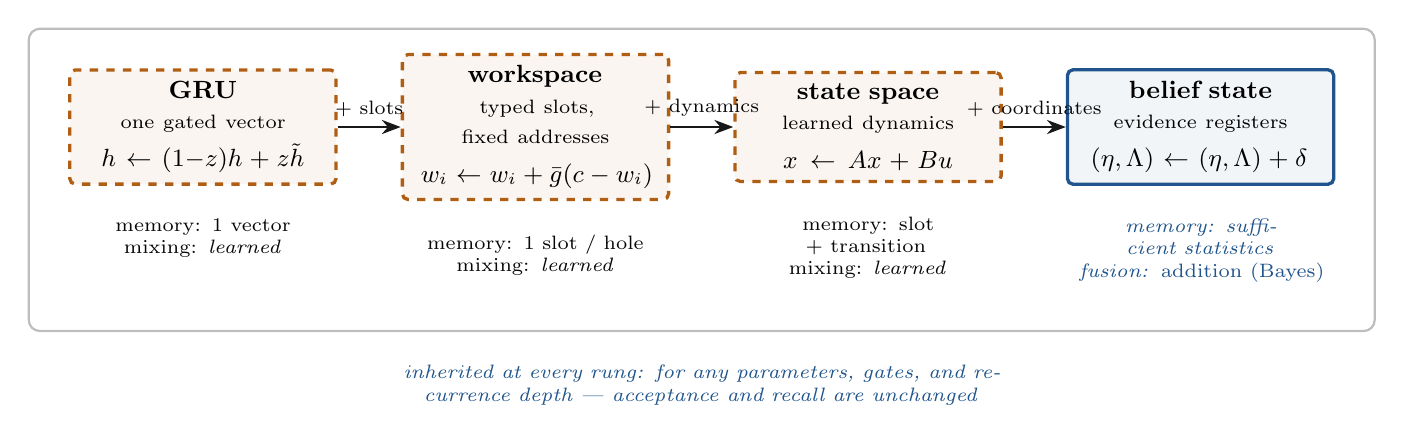
\begin{tikzpicture}[node distance=4mm]

\def\colw{31mm}

\node[learned, text width=\colw] (gru) {\textbf{GRU}\\{\scriptsize one gated vector}\\[1mm]
  $h \leftarrow (1{-}z)h + z\tilde{h}$};
\node[learned, text width=\colw, right=8mm of gru] (ws) {\textbf{workspace}\\{\scriptsize typed slots, fixed addresses}\\[1mm]
  $w_i \leftarrow w_i + \bar{g}(c-w_i)$};
\node[learned, text width=\colw, right=8mm of ws] (ssm) {\textbf{state space}\\{\scriptsize learned dynamics}\\[1mm]
  $x \leftarrow Ax + Bu$};
\node[proved, text width=\colw, right=8mm of ssm] (bel) {\textbf{belief state}\\{\scriptsize evidence registers}\\[1mm]
  $(\eta,\Lambda) \leftarrow (\eta,\Lambda) + \delta$};

\draw[flow] (gru) -- node[lbl, above] {+ slots} (ws);
\draw[flow] (ws) -- node[lbl, above] {+ dynamics} (ssm);
\draw[flow] (ssm) -- node[lbl, above] {+ coordinates} (bel);

\node[lbl, below=3mm of gru, text width=\colw] (c1) {memory: 1 vector\\mixing: \emph{learned}};
\node[lbl, below=3mm of ws, text width=\colw] (c2) {memory: 1 slot / hole\\mixing: \emph{learned}};
\node[lbl, below=3mm of ssm, text width=\colw] (c3) {memory: slot $+$ transition\\mixing: \emph{learned}};
\node[thm, below=3mm of bel, text width=\colw] (c4) {memory: sufficient statistics\\fusion: \emph{addition (Bayes)}};

\begin{scope}[on background layer]
  \node[fit=(gru)(bel)(c1)(c4), draw=datac!40, thick, rounded corners, inner sep=5mm] (box) {};
\end{scope}
\node[thm, below=3mm of box.south, text width=120mm]
  {inherited at every rung: for any parameters, gates, and recurrence depth ---
   acceptance and recall are unchanged};

\end{tikzpicture}}
\caption{The decoder-state ladder. Each rung adds structure and gives away freedom; only
the last replaces learned mixing with the addition Bayes prescribes. The trust boundary
holds identically along the whole ladder, so architecture is a free variable.}
\label{fig:ladder}
\end{figure}

The formal scope of this family is developed in a dedicated Lean tree
(\code{WorkspaceDecoder}, Figure~\ref{fig:ladder}): update~\eqref{eq:workspace} is damped
fixed-point iteration;
under a spectral condition the linear model contracts to a unique equilibrium; and under
finite-depth training mismatch there is a \emph{unique fitted recurrence depth}, with
over-settling strictly worse---so depth is a convergence parameter with an optimum, not
a capacity knob. A prefix-scan theorem (affine transitions form a monoid; scanned
prefixes equal the sequential trajectory) is the correctness license for
parallelizable linear-recurrent variants \cite{gu2023mamba}. A bridge through the
implicit function theorem licenses equilibrium differentiation \cite{bai2019deq} where
the contraction condition holds. Crucially, the trust boundary of
Section~\ref{sec:trust} is inherited: for \emph{any} workspace parameters, gates, and
depth, acceptance and recall are unchanged---the entire architecture axis lives on the
safe side by construction.

\begin{figure}[htbp]
\centering
\resizebox{0.98\textwidth}{!}{%
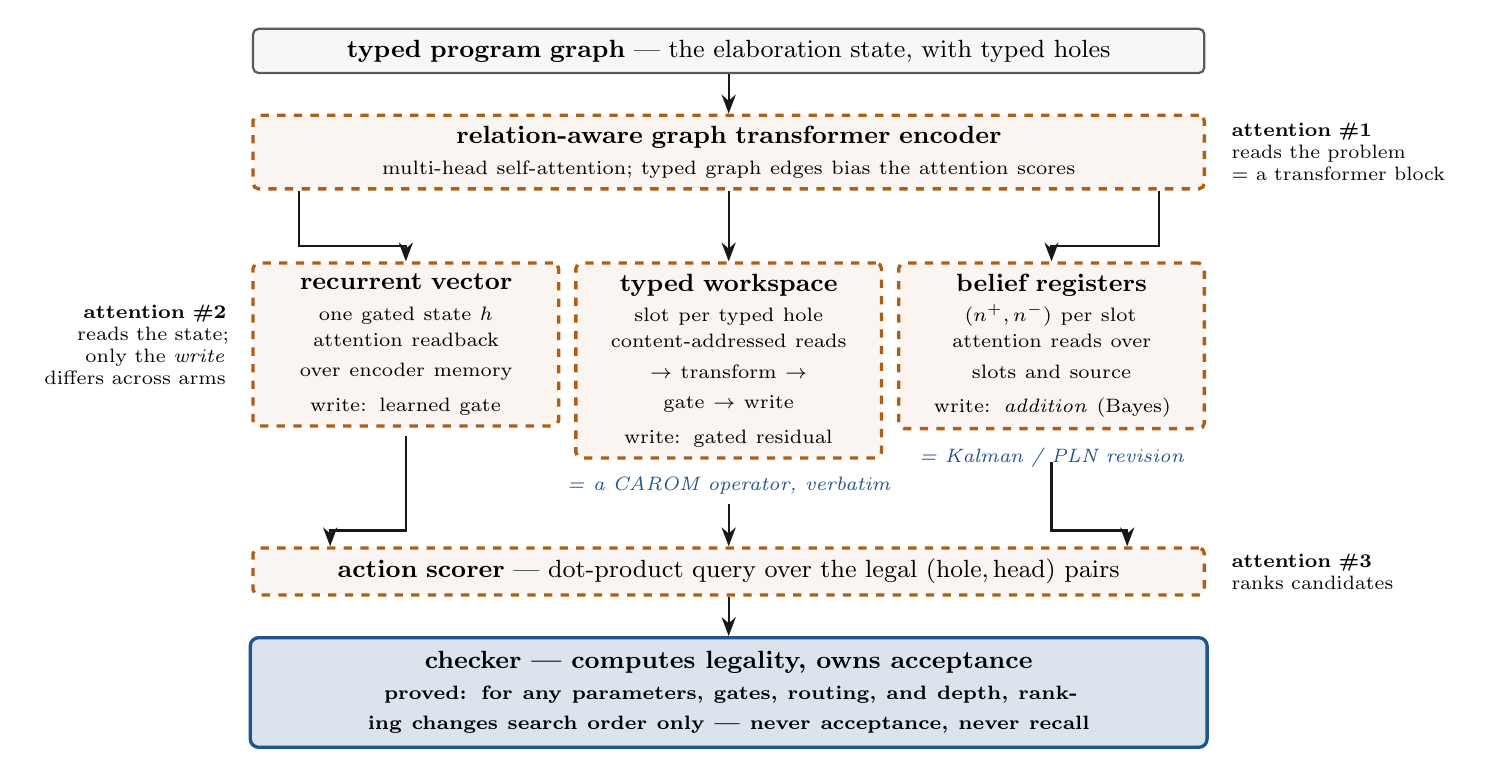
\begin{tikzpicture}[node distance=5mm]

\node[datum, text width=118mm] (graph)
  {\textbf{typed program graph} --- the elaboration state, with typed holes};

\node[learned, text width=118mm, below=5mm of graph] (enc)
  {\textbf{relation-aware graph transformer encoder}\\
   {\scriptsize multi-head self-attention; typed graph edges bias the attention scores}};
\node[lbl, right=2mm of enc.east, text width=30mm, align=left]
  {\textbf{attention \#1}\\reads the problem\\= a transformer block};

% three state carriers
\node[learned, text width=36mm, below=9mm of enc.south west, anchor=north west] (gru)
  {\textbf{recurrent vector}\\{\scriptsize one gated state $h$}\\[0.5mm]
   {\scriptsize attention readback\\over encoder memory}\\[0.5mm]
   {\scriptsize write: learned gate}};
\node[learned, text width=36mm, below=9mm of enc.south] (ws)
  {\textbf{typed workspace}\\{\scriptsize slot per typed hole}\\[0.5mm]
   {\scriptsize content-addressed reads\\$\to$ transform $\to$ gate $\to$ write}\\[0.5mm]
   {\scriptsize write: gated residual}};
\node[learned, text width=36mm, below=9mm of enc.south east, anchor=north east] (bel)
  {\textbf{belief registers}\\{\scriptsize $(n^{+},n^{-})$ per slot}\\[0.5mm]
   {\scriptsize attention reads over\\slots and source}\\[0.5mm]
   {\scriptsize write: \emph{addition} (Bayes)}};
\node[thm, below=1mm of ws.south] (caromlbl) {= a CAROM operator, verbatim};
\node[thm, below=1mm of bel.south] {= Kalman / PLN revision};
\node[lbl, left=2mm of gru.west, text width=24mm, align=right]
  {\textbf{attention \#2}\\reads the state;\\only the \emph{write}\\differs across arms};

\node[learned, text width=118mm, below=11mm of ws] (score)
  {\textbf{action scorer} --- dot-product query over the legal $(\text{hole},\text{head})$ pairs};
\node[lbl, right=2mm of score.east, text width=30mm, align=left]
  {\textbf{attention \#3}\\ranks candidates};

\node[waist, text width=118mm, below=5mm of score] (chk)
  {\textbf{checker} --- computes legality, owns acceptance\\
   {\scriptsize proved: for any parameters, gates, routing, and depth, ranking changes
    search order only --- never acceptance, never recall}};

\draw[flow] (graph) -- (enc);
\draw[flow] (enc.south west) ++(6mm,0) |- ($(gru.north)+(0,2mm)$) -- (gru.north);
\draw[flow] (enc) -- (ws);
\draw[flow] (enc.south east) ++(-6mm,0) |- ($(bel.north)+(0,2mm)$) -- (bel.north);
\draw[flow] (gru.south) ++(0,-1mm) |- ($(score.north west)+(10mm,2mm)$) -- ($(score.north west)+(10mm,0)$);
\draw[flow] (caromlbl.south) -- (score.north);
\draw[flow] (bel.south) ++(0,-4mm) |- ($(score.north east)+(-10mm,2mm)$) -- ($(score.north east)+(-10mm,0)$);
\draw[flow] (score) -- (chk);

\end{tikzpicture}}
\caption{Anatomy of the decoder family, for readers arriving from the transformer world.
Attention is the \emph{read} everywhere: the encoder is a standard multi-head transformer
block whose scores are biased by the typed graph edges; every state carrier reads its
state and the source by content-addressed attention (the workspace's
read--transform--gate--write cycle is exactly a CAROM operator); the action scorer is a
single-head dot-product query. The arms differ only in \emph{write} semantics --- learned
gate, gated residual, or hardwired addition in natural coordinates --- which is the
decoder-state ladder of Figure~\ref{fig:ladder} seen mechanically. The checker sits below
everything: legality and acceptance are computed outside the network, so the entire
learned stack can only reorder search.}
\label{fig:anatomy}
\end{figure}

\begin{figure}[htbp]
\centering
\resizebox{0.99\textwidth}{!}{%
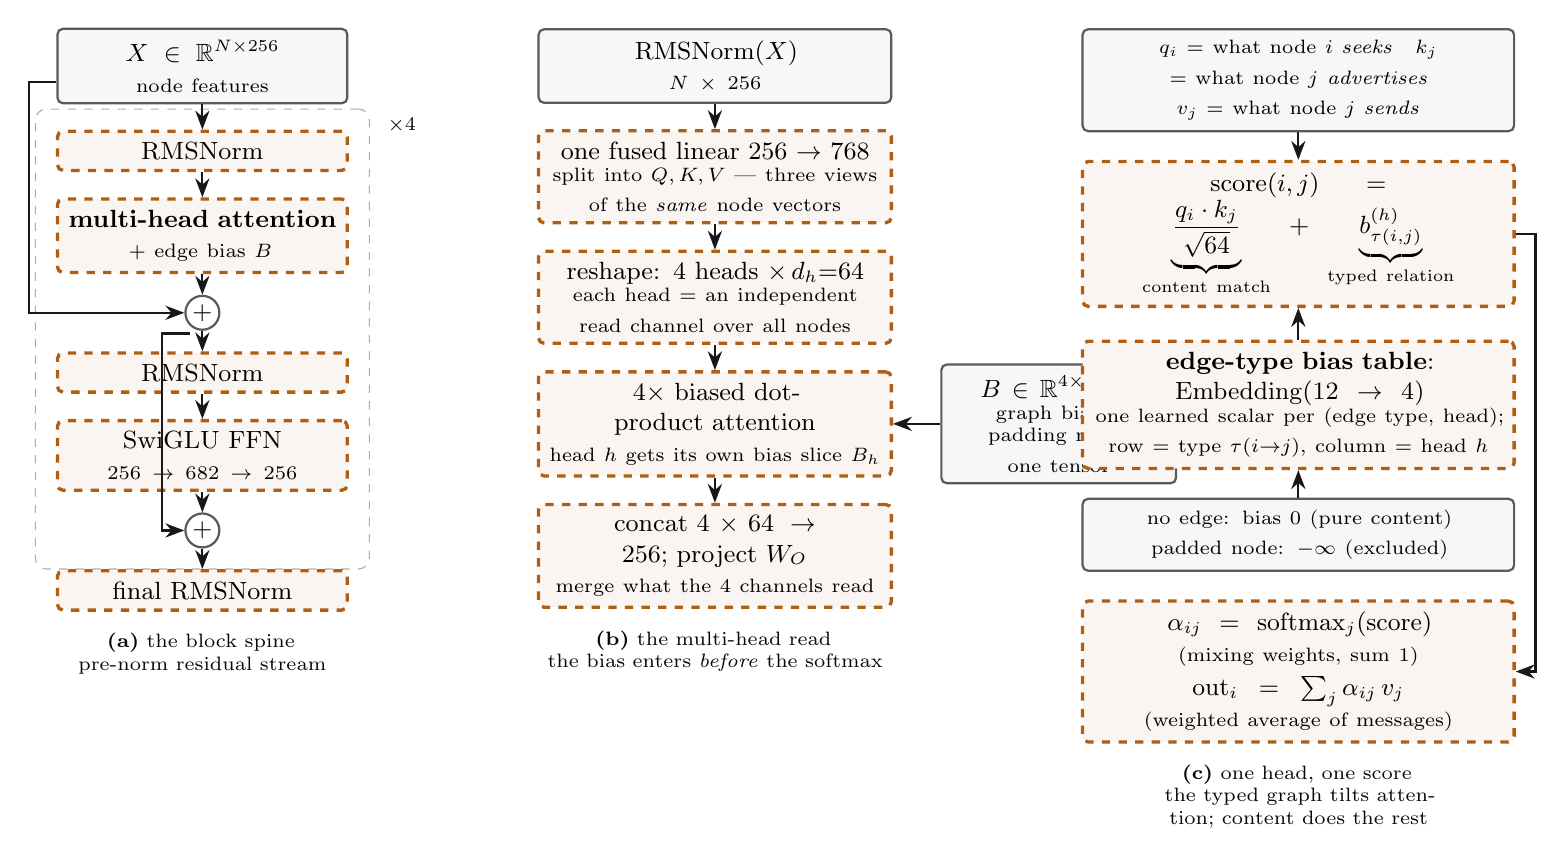
\begin{tikzpicture}[node distance=3.2mm, every node/.style={font=\small}]

% ---------- panel (a): block spine ----------
\node[datum, text width=34mm] (aX) {$X \in \mathbb{R}^{N\times 256}$\\{\scriptsize node features}};
\node[learned, text width=34mm, below=of aX] (an1) {RMSNorm};
\node[learned, text width=34mm, below=of an1] (aatt) {\textbf{multi-head attention}\\{\scriptsize $+$ edge bias $B$}};
\node[circle, draw=datac, thick, inner sep=1pt, below=2.6mm of aatt] (aplus1) {$+$};
\node[learned, text width=34mm, below=2.6mm of aplus1] (an2) {RMSNorm};
\node[learned, text width=34mm, below=of an2] (affn) {SwiGLU FFN\\{\scriptsize $256 \to 682 \to 256$}};
\node[circle, draw=datac, thick, inner sep=1pt, below=2.6mm of affn] (aplus2) {$+$};
\node[learned, text width=34mm, below=2.6mm of aplus2] (afin) {final RMSNorm};
\draw[flow] (aX) -- (an1);
\draw[flow] (an1) -- (aatt);
\draw[flow] (aatt) -- (aplus1);
\draw[flow] (aplus1) -- (an2);
\draw[flow] (an2) -- (affn);
\draw[flow] (affn) -- (aplus2);
\draw[flow] (aplus2) -- (afin);
\draw[flow] (aX.west) ++(0,-2mm) -- ++(-3.5mm,0) |- (aplus1.west);
\draw[flow] (aplus1.south west) ++(0,-1mm) -- ++(-3.5mm,0) |- (aplus2.west);
\begin{scope}[on background layer]
  \node[fit=(an1)(aplus2), draw=datac!50, dashed, rounded corners, inner sep=2.6mm] (ablock) {};
\end{scope}
\node[lbl, right=1mm of ablock.north east, anchor=north west] {$\times 4$};
\node[lbl, below=1.5mm of afin, text width=36mm] {\textbf{(a)} the block spine\\{\scriptsize pre-norm residual stream}};

% ---------- panel (b): multi-head with bias injection ----------
\node[datum, text width=42mm, right=24mm of aX] (bX) {$\mathrm{RMSNorm}(X)$\\{\scriptsize $N\times 256$}};
\node[learned, text width=42mm, below=of bX] (bqkv) {one fused linear $256 \to 768$\\{\scriptsize split into $Q, K, V$ --- three views\\of the \emph{same} node vectors}};
\node[learned, text width=42mm, below=of bqkv] (bsplit) {reshape: $4$ heads $\times\, d_h{=}64$\\{\scriptsize each head = an independent\\read channel over all nodes}};
\node[learned, text width=42mm, below=of bsplit] (bheads) {$4\times$ biased dot-product attention\\{\scriptsize head $h$ gets its own bias slice $B_h$}};
\node[learned, text width=42mm, below=of bheads] (bcat) {concat $4\times 64 \to 256$;\ project $W_O$\\{\scriptsize merge what the 4 channels read}};
\node[datum, text width=27mm, right=6mm of bheads] (bbias) {$B \in \mathbb{R}^{4\times N\times N}$\\{\scriptsize graph bias $+$\\padding mask,\\one tensor}};
\draw[flow] (bX) -- (bqkv);
\draw[flow] (bqkv) -- (bsplit);
\draw[flow] (bsplit) -- (bheads);
\draw[flow] (bheads) -- (bcat);
\draw[flow] (bbias) -- (bheads);
\node[lbl, below=1.5mm of bcat, text width=44mm] {\textbf{(b)} the multi-head read\\{\scriptsize the bias enters \emph{before} the softmax}};

% ---------- panel (c): one head, one score ----------
\node[datum, text width=52mm, right=24mm of bX.north east, anchor=north west] (cqkv)
  {{\scriptsize $q_i$ = what node $i$ \emph{seeks}\quad
    $k_j$ = what node $j$ \emph{advertises}\quad
    $v_j$ = what node $j$ \emph{sends}}};
\node[learned, text width=52mm, below=3.5mm of cqkv] (cq)
  {score$(i,j) \;=\; \underbrace{\dfrac{q_i \cdot k_j}{\sqrt{64}}}_{\text{content match}} \;+\; \underbrace{b^{(h)}_{\tau(i,j)}}_{\text{typed relation}}$};
\node[learned, text width=52mm, below=4mm of cq] (ctab)
  {\textbf{edge-type bias table}: $\mathrm{Embedding}(12 \to 4)$\\{\scriptsize one learned scalar per (edge type, head);\\row $=$ type $\tau(i{\to}j)$, column $=$ head $h$}};
\node[datum, text width=52mm, below=3.5mm of ctab] (cnil)
  {{\scriptsize no edge: bias $0$ (pure content) \quad padded node: $-\infty$ (excluded)}};
\node[learned, text width=52mm, below=3.5mm of cnil] (csoft)
  {$\alpha_{ij} = \mathrm{softmax}_j(\text{score})$ \ {\scriptsize (mixing weights, sum $1$)}\\[0.5mm]
   $\mathrm{out}_i = \textstyle\sum_j \alpha_{ij}\, v_j$ \ {\scriptsize (weighted average of messages)}};
\draw[flow] (cqkv) -- (cq);
\draw[flow] (ctab) -- (cq);
\draw[flow] (cnil) -- (ctab);
\draw[flow] (cq.east) -- ++(2.5mm,0) |- (csoft.east);
\node[lbl, below=1.5mm of csoft, text width=52mm] {\textbf{(c)} one head, one score\\{\scriptsize the typed graph tilts attention; content does the rest}};

\end{tikzpicture}}
\caption{Zooming into the encoder of Figure~\ref{fig:anatomy}, innermost panel last ---
self-contained, so the transformer itself can be read off, not just our variant.
\textbf{(a)} The residual stream: each of four blocks \emph{adds} a refinement to the
running node representations rather than replacing them (the $+$ junctions), with
normalization \emph{before} each sublayer (pre-norm; RMS scaling only, no mean
subtraction) and a gated position-wise feed-forward (SwiGLU) that processes every node
independently. \textbf{(b)} Multi-head attention: one linear map makes three views of
each node vector --- queries, keys, values --- split across four independent
$64$-dimensional read channels; the $\sqrt{64}$ keeps scores in softmax's useful range.
Rotary position (RoPE) is applied to $Q,K$ by \emph{node index}, which is meaningful
order on the sequence path and incidental on derived/global nodes --- graph structure is
carried by the bias, not by position. \textbf{(c)} The one departure from a vanilla
transformer, after Graphormer: each head's score is content match \emph{plus} a learned
scalar for the typed relation between the two nodes, from a $12\times 4$ table. No edge
means bias zero --- the encoder degrades gracefully to a set transformer --- and the
padding mask rides in the same tensor as $-\infty$ columns. Everything the model knows
about the graph enters through these $48$ numbers.}
\label{fig:encoderzoom}
\end{figure}

\begin{figure}[htbp]
\centering
\resizebox{0.99\textwidth}{!}{%
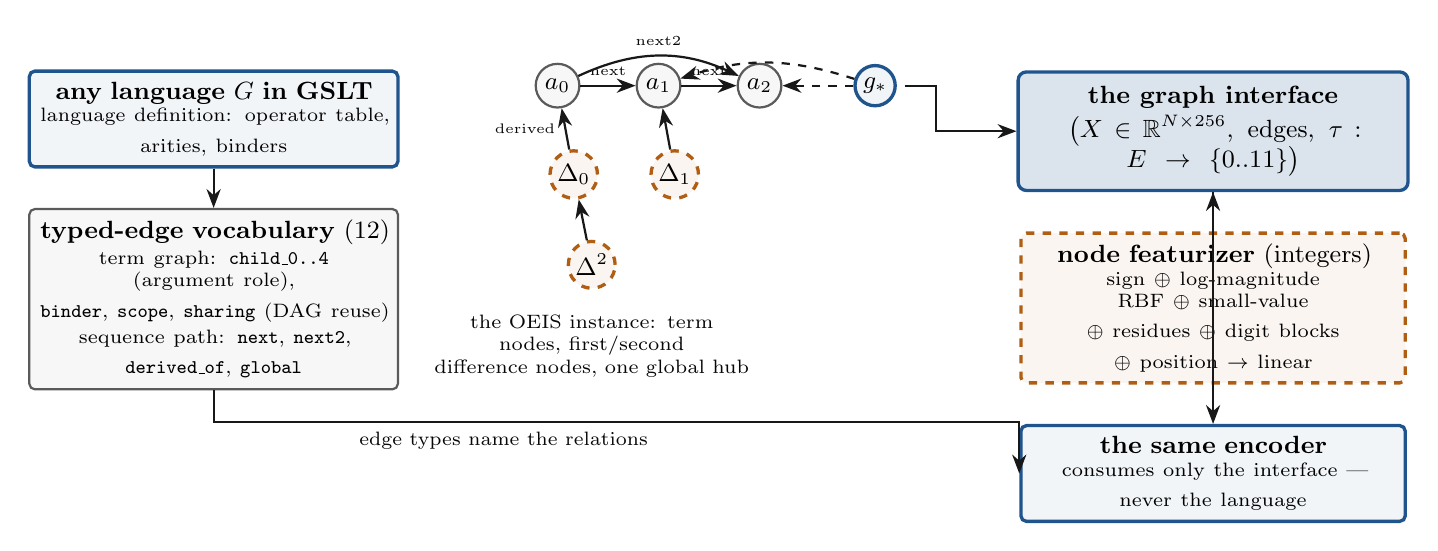
\begin{tikzpicture}[node distance=4mm, every node/.style={font=\small}]

% ---- left: the GSLT-generic vocabulary ----
\node[proved, text width=44mm] (lang)
  {\textbf{any language $G$ in GSLT}\\{\scriptsize language definition: operator table,\\arities, binders}};
\node[datum, text width=44mm, below=5mm of lang] (vocab)
  {\textbf{typed-edge vocabulary} (12)\\[0.5mm]
   {\scriptsize term graph: \code{child\_0..4} (argument role),\\ \code{binder}, \code{scope}, \code{sharing} (DAG reuse)}\\[0.5mm]
   {\scriptsize sequence path: \code{next}, \code{next2},\\ \code{derived\_of}, \code{global}}};
\draw[flow] (lang) -- (vocab);

% ---- middle: the OEIS instance graph ----
\node[datum, circle, inner sep=2pt, right=18mm of lang.north east, anchor=north west] (t0) {$a_0$};
\node[datum, circle, inner sep=2pt, right=7mm of t0] (t1) {$a_1$};
\node[datum, circle, inner sep=2pt, right=7mm of t1] (t2) {$a_2$};
\node[learned, circle, inner sep=1.2pt, below=6mm of t0.south east] (d0) {$\Delta_0$};
\node[learned, circle, inner sep=1.2pt, below=6mm of t1.south east] (d1) {$\Delta_1$};
\node[learned, circle, inner sep=1pt, below=6mm of d0.south east] (dd) {$\Delta^2$};
\node[proved, circle, inner sep=1.5pt, right=9mm of t2] (glob) {$g_\ast$};
\draw[flow] (t0) -- node[lbl, above] {\tiny next} (t1);
\draw[flow] (t1) -- node[lbl, above] {\tiny next} (t2);
\draw[flow, bend left=25] (t0) to node[lbl, above] {\tiny next2} (t2);
\draw[flow] (d0) -- node[lbl, left] {\tiny derived} (t0);
\draw[flow] (d1) -- (t1);
\draw[flow] (dd) -- (d0);
\draw[flow, dashed] (glob) -- (t2);
\draw[flow, dashed, bend right=18] (glob) to (t1);
\node[lbl, below=2mm of dd, text width=48mm]
  {the OEIS instance: term nodes, first/second\\difference nodes, one global hub};

% ---- right: the interface ----
\node[waist, text width=46mm, right=16mm of glob.north east, anchor=north west] (iface)
  {\textbf{the graph interface}\\[0.5mm]
   $\bigl(X \in \mathbb{R}^{N\times 256},\ \mathrm{edges},\ \tau : E \to \{0..11\}\bigr)$};
\node[learned, text width=46mm, below=5mm of iface] (feats)
  {\textbf{node featurizer} (integers)\\{\scriptsize sign $\oplus$ log-magnitude RBF $\oplus$ small-value\\ $\oplus$ residues $\oplus$ digit blocks $\oplus$ position $\to$ linear}};
\node[proved, text width=46mm, below=5mm of feats] (enc)
  {\textbf{the same encoder}\\{\scriptsize consumes only the interface ---\\never the language}};
\draw[flow] (feats) -- (iface);
\draw[flow] (iface) -- (enc.north);
\draw[flow] (glob.east) ++(1mm,0) -- ++(4mm,0) |- (iface.west);
\draw[flow] (vocab.south) -- ++(0,-4mm) -| node[lbl, pos=0.18, below] {\scriptsize edge types name the relations} (enc.west) {};

\end{tikzpicture}}
\caption{Why the encoder works for any graph $g$ of any language $G$ in GSLT. A language
definition induces term graphs over a fixed typed-relation vocabulary --- argument-role
edges \code{child\_k}, \code{binder}/\code{scope} for variable structure, \code{sharing}
for DAG reuse --- and a problem instance contributes its own relations (here: the OEIS
sequence path with difference nodes and a global hub). Everything is compiled down to one
interface: node feature vectors, an edge list, and an edge-type map. The encoder is
defined on that interface alone, so changing the language changes the graph, never the
network; legality and typing live in the checker's mask, outside the learned stack.}
\label{fig:graphinterface}
\end{figure}

\subsection{Fusion is addition; charts are shadows}
\label{sec:fusion}

The crown of the state theory is a single identity. Write belief in \emph{natural
coordinates}: evidence counts $(n^{+},n^{-})$ in the discrete case
\cite{pln2009}, the information form $(\eta,\Lambda)=(\Sigma^{-1}\mu,\Sigma^{-1})$ in
the Gaussian case. Then:
\begin{itemize}
\item Bayesian fusion of independent evidence is \emph{addition} in natural
coordinates---componentwise for counts, matrix addition for information;
\item the Kalman update, the gated-interpolation step~\eqref{eq:workspace}, and
probabilistic-logic revision are the \emph{same} addition, viewed after normalizing to
the moment chart; the optimal gate is the Kalman gain, and the workspace equilibrium
under exact gains is the Bayesian posterior mean
(\code{equilibrium\_iff\_eq\_posteriorMean});
\item strength and confidence are derived columns of the counts, recovered by the
sealed confidence characterization; the counts are the sufficient statistics and the
primal state.
\end{itemize}
The identity is a commuting square (Figure~\ref{fig:fusion}): fusion is addition
upstairs; every gated-interpolation rule anyone has ever hand-designed is that same
addition seen downstairs, after normalizing to the moment chart.

\begin{figure}[htbp]
\centering
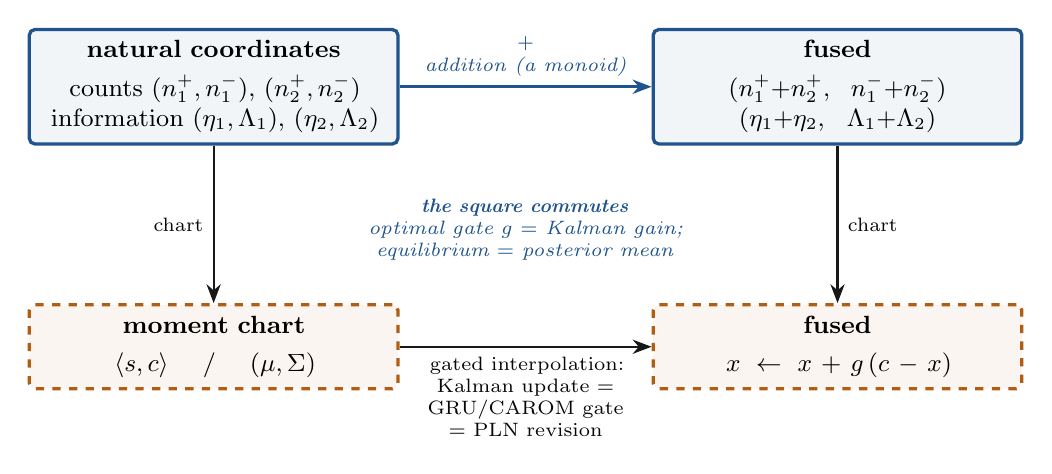
\begin{tikzpicture}[node distance=6mm]

\node[proved, text width=44mm] (nat1) {\textbf{natural coordinates}\\[1mm]
  counts $(n^{+}_1,n^{-}_1),\,(n^{+}_2,n^{-}_2)$\\
  information $(\eta_1,\Lambda_1),\,(\eta_2,\Lambda_2)$};
\node[proved, text width=44mm, right=32mm of nat1] (nat2) {\textbf{fused}\\[1mm]
  $(n^{+}_1{+}n^{+}_2,\; n^{-}_1{+}n^{-}_2)$\\
  $(\eta_1{+}\eta_2,\; \Lambda_1{+}\Lambda_2)$};

\node[learned, text width=44mm, below=20mm of nat1] (mom1) {\textbf{moment chart}\\[1mm]
  $\langle s,c\rangle$ \quad / \quad $(\mu,\Sigma)$};
\node[learned, text width=44mm, below=20mm of nat2] (mom2) {\textbf{fused}\\[1mm]
  $x \leftarrow x + g\,(c - x)$};

\draw[flow, provedc, very thick] (nat1) -- node[thm, above] {$+$\\\scriptsize addition (a monoid)} (nat2);
\draw[flow] (mom1) -- node[lbl, below, text width=44mm] {gated interpolation:\\Kalman update $=$ GRU/CAROM gate\\$=$ PLN revision} (mom2);
\draw[flow] (nat1) -- node[lbl, left] {chart} (mom1);
\draw[flow] (nat2) -- node[lbl, right] {chart} (mom2);

\node[thm, below=13mm of $(nat1)!0.5!(nat2)$, text width=52mm]
  {\textbf{the square commutes}\\
   optimal gate $g$ $=$ Kalman gain;\\
   equilibrium $=$ posterior mean};

\end{tikzpicture}
\caption{Fusion is addition; charts are shadows. Three rules invented independently in
three literatures --- Kalman filtering, gated recurrence, probabilistic-logic revision
--- are one operation, and it is only nonlinear because the moment chart is.}
\label{fig:fusion}
\end{figure}

Sequentially, Riccati covariance propagation makes the optimal gain time-varying, and a
sharp condition ($R_2(P+R_1)\neq R_1^2$ in the scalar case) implies every
\emph{constant} gate is strictly suboptimal---the derived reason input-conditioned
gating (``selectivity'') earns its complexity.

This licenses a concrete cell (Figure~\ref{fig:cell}): slots hold additive evidence
registers; learned operators propose \emph{measurements} (what observations mean); a
learned gain network, conditioned on the slot's own precision, scales them; the state
update is pure addition; readout charts to moments and scores only legal actions.
Everything Bayes determines (how to fuse) is hardwired; everything Bayes leaves open
(what observations mean, what the noise is) is learned.

\begin{figure}[htbp]
\centering
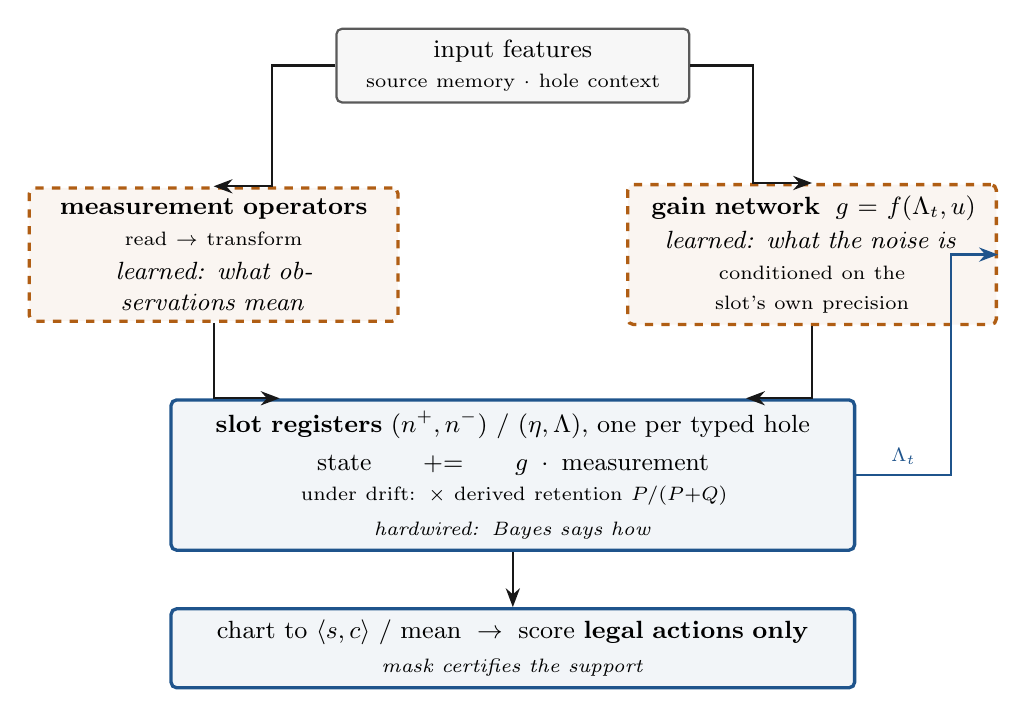
\begin{tikzpicture}

\node[datum, text width=42mm] (in) at (0,0)
  {input features\\{\scriptsize source memory $\cdot$ hole context}};

\node[learned, text width=44mm] (ops) at (-38mm,-24mm)
  {\textbf{measurement operators}\\{\scriptsize read $\to$ transform}\\[0.5mm]
   \emph{learned: what observations mean}};
\node[learned, text width=44mm] (gain) at (38mm,-24mm)
  {\textbf{gain network}\; $g = f(\Lambda_t, u)$\\[0.5mm]
   \emph{learned: what the noise is}\\
   {\scriptsize conditioned on the slot's own precision}};

\node[proved, text width=84mm] (state) at (0,-52mm)
  {\textbf{slot registers} $(n^{+},n^{-})$ / $(\eta,\Lambda)$, one per typed hole\\[1mm]
   $\text{state} \;\mathrel{+}=\; g \cdot \text{measurement}$\\
   {\scriptsize under drift: $\times$ derived retention $P/(P{+}Q)$}\\[0.5mm]
   {\scriptsize\itshape hardwired: Bayes says how}};

\node[proved, text width=84mm] (out) at (0,-74mm)
  {chart to $\langle s,c\rangle$ / mean \;$\to$\; score \textbf{legal actions only}\\[0.5mm]
   {\scriptsize\itshape mask certifies the support}};

\draw[flow] (in.west) -- ++(-8mm,0) |- (ops.north);
\draw[flow] (in.east) -- ++(8mm,0) |- (gain.north);
\draw[flow] (ops.south) |- ($(state.north west)+(14mm,0)$);
\draw[flow] (gain.south) |- ($(state.north east)+(-14mm,0)$);
\draw[flow] (state) -- (out);
% precision feedback to the gain network
\draw[flow, provedc] (state.east) -- ++(12mm,0)
  node[thm, midway, above] {$\Lambda_t$} |- (gain.east);

\end{tikzpicture}
\caption{The cell the theorems license. Learning concentrates where Bayes is silent ---
in the measurement maps and the gain schedule --- while fusion itself is the addition
Bayes prescribes. The precision register feeds the gain network, which is what makes
selectivity possible; the readout can only rank actions the checker already admits.}
\label{fig:cell}
\end{figure}

\subsection{Where hardwiring is provably wrong: the open world}
\label{sec:openworld}

The optimality of hardwired addition is conditional, and each condition fails somewhere
we care about. Addition never forgets: confidence is monotone in accumulated evidence.
Under drift---a world whose parameters move---monotone accumulation is \emph{provably}
suboptimal; the optimal filter fades memory, and the correct decay rate is derived from
the drift statistics, not tuned. Naive addition double-counts correlated re-observation.
A single natural-coordinate slot projects away multimodal posteriors. And a
miscalibrated measurement model poisons exact fusion, where a learned mixer could have
compensated.

We take an explicit position: \emph{optimizing for the closed world is the wrong
default}. Worlds drift; open-world probabilistic-logic systems build forgetting in for
good reason. Mathematical domains---the OEIS loop below, proof search---are the
distinguished near-stationary regimes where hardwired fusion may legitimately excel,
and that is precisely why they are the right first battleground: if structure cannot
win \emph{there}, it wins nowhere.

The boundary theory is now sealed, and each failure mode is a theorem with a formula.
\emph{Nesting}: precision addition realizes exactly the interpolation gates $[0,1)$ of
the learned-mixing family, and the unit-gate complement splits cleanly into observation
discount, strict old-evidence decay, and overwrite---the precise freedoms hardwired
fusion lacks. \emph{Double counting}: naive addition overstates precision by exactly
the declared evidence overlap, in closed form, and a discounted fusion (proved also
count-natively) restores calibration. \emph{Drift}: in the jump model
$P\mapsto P+Q$, every accumulator whose effective variance stays $\le P$ under-gains and
carries strictly greater risk whenever $Q>0$; the derived old-information retention is
$P/(P+Q)$, moment retention $R/(P+Q+R)$, repeated updates fade exponentially, and
$Q=0$ recovers stationary addition---forgetting as a \emph{derived rate}, not an
aesthetic. \emph{Miscalibration}: for a distorted measurement $y=dx+\varepsilon$,
learned mixing strictly beats the uncorrected unit-model rule exactly off the boundary
$(d-1)(Pd-R)=0$; but recalibrating the measurement map ($y\mapsto y/d$,
$R\mapsto R/d^{2}$) reproduces the same optimal update with fusion left hardwired---and
against the \emph{true}-model gain, learned mixing cannot win at all, since that gain
is already optimal. Every fusion-stage repair thus relocates to the measurement map.

The design conclusion is not ``hardwire everything'' but \emph{learning is necessary,
and theorems say where}: in the measurement maps, in the gain schedules, and---under
drift---in a decay whose rate the jump statistics determine, while fusion itself
remains addition wherever stationarity survives contact with the domain. Each theorem
doubles as a pre-registered diagnostic: whether a learned arm's advantage comes from
forgetting, observation discount, dependence repair, or measurement recalibration is
identifiable from the per-slot trajectories the experiment schema already carries. One
implementation obligation follows: fractional forgetting requires an honest
weighted-evidence layer---it is not to be smuggled into natural-number counts.

\subsection{Routing, order, and the switching boundary}
\label{sec:routing}

The workspace family has a natural command-driven refinement (personal communication,
2026): a small vocabulary of opaque command tokens, softmax-routed over $K$ reusable
read--transform--gate--write experts, with slot state split into an immutable evidence
field, a fixed positional code, and the evolving contents that
update~\eqref{eq:workspace} governs. Four boundary theorems now frame what routing can
and cannot add.

\emph{Routing stays on the ladder.} A simplex mixture of gated-interpolation experts is
again a single gated interpolation under the mixed gain
(\code{mixedExpertStep\_eq\_singleInterpolation}), so routing buys input-conditioned
selectivity---which the Riccati argument above already priced as necessary---without
leaving the update class; and the immutable evidence field survives every routing
schedule, temperature, and depth (\code{runTripleSlotSchedule\_evidence}). Command
tokens themselves carry no semantics: trajectories are determined by the induced
routing schedule alone (\code{commandTrajectory\_eq\_of\_mixtureSchedule\_eq}), and
distinct tokens with equal routes are behaviorally indistinguishable. Meaning lives in
routes, not names.

\emph{Compositionality is commutation.} When are two command phases order-independent,
so that a schedule is a \emph{set} of edits rather than a brittle sequence? For affine
phases the answer is exact: swapping the order shifts the state by
$[B,A]\,x + (Ba + b - Ab - a)$ (\code{affineCompositionDiscrepancy\_exact}), and
order-independence holds iff the linear parts commute \emph{and} the affine obstruction
vanishes (\code{affinePhases\_orderIndependent\_iff}); commuting linear parts alone are
not enough---a one-dimensional bias counterexample closes that loophole. Equivalently,
the pairwise interference energy $\lVert[A,B]\rVert_F^{2}$ must vanish
(\code{linearPhases\_orderIndependent\_iff\_interferenceEnergy\_zero})---a Gram
diagnostic computable from any trained operator pair. Compositionality thereby stops
being an emergent hope and becomes a measured certificate.

\emph{Stability does not compose.} Two commands, each individually
extinguishing---either alone reaches rest in two steps---alternate to $4^{n}$ growth
(\code{individuallyStable\_switchingDiverges}). Per-command guarantees are therefore
worthless for command \emph{programs}; the honest certificate is schedule-uniform. A
common quadratic Lyapunov function bounds every schedule at one geometric rate, and
commuting stable generators always admit one
(\code{commutingCommonQuadraticLyapunov\_crown}). A command-driven decoder should ship
with a switching certificate, not a per-command one.

\emph{Safety is indifferent to all of it.} The trust boundary extends verbatim: for
arbitrary routes, temperatures, schedules, and depths, ranked acceptance coincides with
checker acceptance and recall of accepted programs is unchanged
(\code{inheritanceCrown}). The routing axis, like the state axis, lives entirely on the
safe side; the theorems above are about competence, not safety.

When trained operators cannot be made to commute, there is a second, older route to
order-independence: canonicalize. Interleave the learned step with a projection onto
canonical forms, $s_{t+1} = \mathrm{canon}(f_{\phi}(s_t, c_t))$, and order-sensitivity
is quotiented away rather than trained away: a confluent canonicalizer sends both
orders of a critical pair to one normal form---exactly the commutation the raw
operators lack---while the per-step projection stops representational drift from
compounding across a schedule. The iterated form is a weight-tied loop of the same
transformer, the regime in which looped transformers act as programmable
computers~\cite{giannou2023}; canonicalization is the projection that keeps the loop's
state on the quotient. This program already runs on that principle at two other
scales: the determinism lemma of Section~\ref{sec:waist} is the confluence statement
for spine creation, and canonical-forms $LF$ makes conversion vanish into the syntax.
The design conclusion repeats itself one level up: learn the proposal, hardwire the
quotient.

\section{The loop compounds, and the factorial that kept us honest}
\label{sec:experiments}

The empirical instance is cumulative self-improvement on OEIS program discovery
\cite{gauthier2023} (Figure~\ref{fig:loop}): train on the accumulated verified corpus,
search under fixed budgets, check every candidate against the whole encyclopedia, add
what verifies, repeat. The same wake--sleep shape drives other self-improving synthesis
systems, which additionally distil reusable abstractions into the library between rounds
\cite{ellis2021}; here the checker plays the role of the sleep-phase filter, and the
waist fixes what a reusable action is.

\begin{figure}[htbp]
\centering
\resizebox{\textwidth}{!}{%
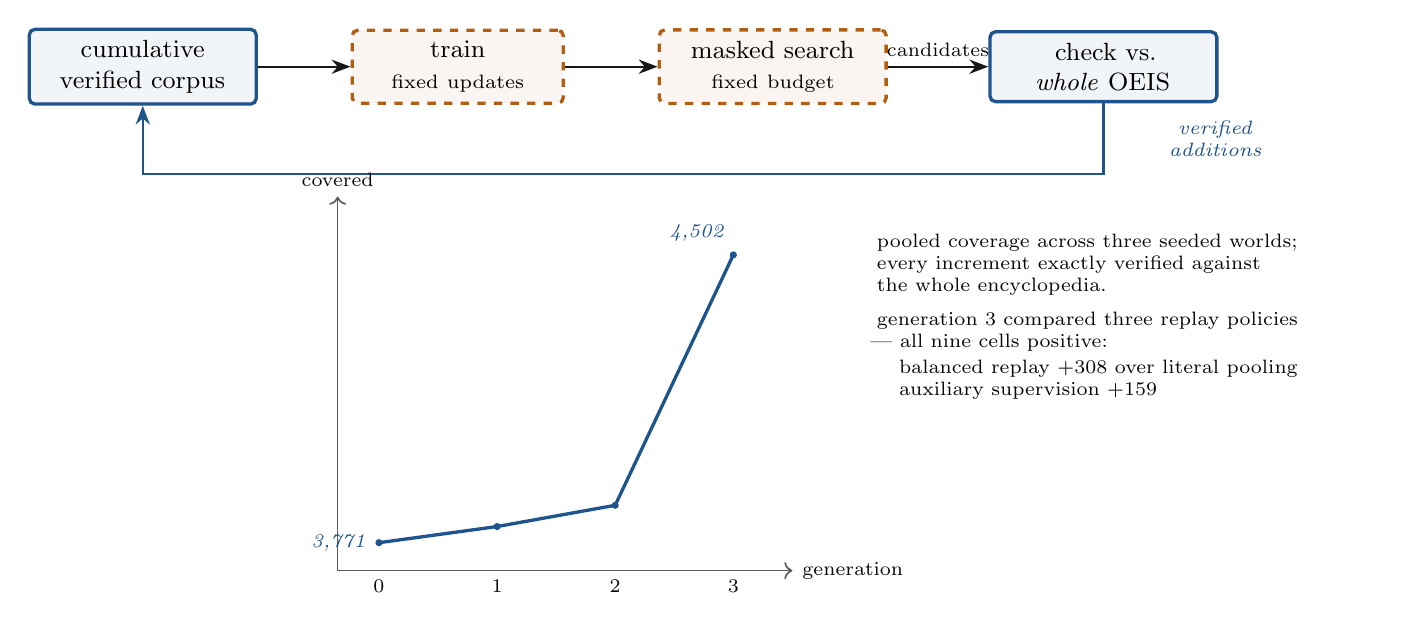
\begin{tikzpicture}

% ---- the loop (top row) ----
\node[proved, text width=26mm] (corpus) at (0,0) {cumulative\\verified corpus};
\node[learned, text width=24mm] (train) at (40mm,0) {train\\{\scriptsize fixed updates}};
\node[learned, text width=26mm] (search) at (80mm,0) {masked search\\{\scriptsize fixed budget}};
\node[proved, text width=26mm] (check) at (122mm,0) {check vs.\\\emph{whole} OEIS};

\draw[flow] (corpus) -- (train);
\draw[flow] (train) -- (search);
\draw[flow] (search) -- node[lbl, above] {candidates} (check);
\draw[flow, provedc] (check.south) -- ++(0,-9mm)
   node[thm, midway, right, text width=26mm] {verified\\additions}
   -| (corpus.south);

% ---- the trajectory (below), plotted in offset units: value - 3700 ----
\begin{scope}[shift={(30mm,-64mm)}, x=15mm, y=0.05mm]
  \draw[->, semithick, draw=datac] (-0.35,0) -- (3.5,0) node[lbl, right] {generation};
  \draw[->, semithick, draw=datac] (-0.35,0) -- (-0.35,950) node[lbl, above] {covered};
  \draw[very thick, provedc] (0,71) -- (1,112) -- (2,166) -- (3,802);
  \foreach \g/\c in {0/71, 1/112, 2/166, 3/802} { \fill[provedc] (\g,\c) circle (1.3pt); }
  \foreach \g in {0,1,2,3} { \node[lbl, below] at (\g,0) {\g}; }
  \node[thm, left=0.5mm] at (0,71) {3{,}771};
  \node[thm, above left=0.5mm and 0mm] at (3,802) {4{,}502};
\end{scope}

\node[lbl, text width=64mm, align=left, anchor=north west] at (92mm,-20mm)
  {pooled coverage across three seeded worlds;\\
   every increment exactly verified against\\
   the whole encyclopedia.\\[1.5mm]
   generation~3 compared three replay policies\\
   --- all nine cells positive:\\[0.5mm]
   \quad balanced replay $+308$ over literal pooling\\
   \quad auxiliary supervision $+159$};

\end{tikzpicture}}
\caption{The loop compounds. At literal pooling the model's own discoveries carry
$0.24\%$ of sampling mass and the loop starves on the signal it exists to generate;
balanced replay is what makes self-improvement visible.}
\label{fig:loop}
\end{figure} Three independently seeded worlds grew coverage from a shared initial
$3{,}771$ known sequences to $3{,}986$ after two generations, and---under a
prospectively registered three-way comparison of replay policies at generation
three---to $4{,}502$ before generation four, with all nine cells positive. Balanced
replay of the model's own discoveries ($25\%$ mass) beat literal pooling by $+308$
pooled sequences: at natural sampling mass ($0.24\%$), the loop starves on exactly the
signal it exists to generate. Auxiliary predictive supervision added $+159$. The union
of generation-three discoveries was $503$ distinct sequences, for $697$ verified
model-origin programs accumulated by generation four.

Two registered negatives bound the claims. An ablation asking whether a world's own
discoveries beat an equal mass of \emph{unused external} certified data answers
no---but that comparator does not exist in the deployed regime, where the corpus is
whatever the loop has verified; it is an oracle-advantaged ablation, not the loop
objective. And no arm, in any generation, solved its own assigned held-out target
within budget: the evidence concerns learned \emph{discovery} guidance over the
catalogue, not target-conditioned synthesis.

A twelve-cell factorial (decoder architecture $\times$ auxiliary supervision $\times$
three seeds) disentangled an earlier confound: a one-seed comparison had suggested a
token-sequence decoder beat the typed-action decoder $38$--$28$; the factorial showed
the apparent gap was carried by asymmetric auxiliary supervision, and across seeds the
typed-action decoder led pooled ($188$ vs.\ $119$, positive in $2/3$ seeds) with the
supervision interaction inconsistent---no interaction claim survives. One-seed
architecture stories, in this regime, are noise until replicated.

The registered comparison the state theory now sharpens is three-lineage: the gated
recurrent incumbent, the typed workspace (learned mixing, CAROM-style), and the
belief-state cell (hardwired fusion)---matched capacity, identical trunks warm-started
and decoder-specific parameters reinitialized, two further cumulative generations,
per-slot evidence trajectories logged in a pinned schema, and the interpretation bins
written before launch. A parallel $2\times2$ tests a shallow predictive-coding residual
adapter over \emph{both} backbone architectures; the interaction contrast is the
estimand, and the settling theory predicts the workspace backbone is where a local
settling rule has its best chance.

\section{The same waist, pointed outward}
\label{sec:ladder-out}

Because the interface is root-parametric, pointing it at a new language is an
instantiation, not a rewrite. Pointed at an external dependent-type inhabitation
benchmark \cite{norman2026}, the authentication gate became a measuring instrument for
the benchmark itself (Figure~\ref{fig:roots}):

\begin{figure}[htbp]
\centering
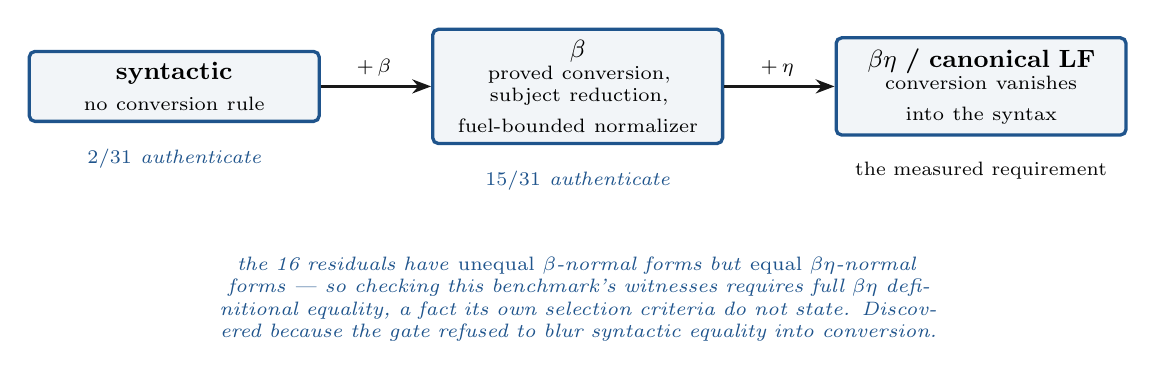
\begin{tikzpicture}[node distance=6mm]

\node[proved, text width=34mm] (syn) {\textbf{syntactic}\\{\scriptsize no conversion rule}};
\node[proved, text width=34mm, right=14mm of syn] (beta) {\textbf{$\beta$}\\{\scriptsize proved conversion,\\subject reduction,\\fuel-bounded normalizer}};
\node[proved, text width=34mm, right=14mm of beta] (eta) {\textbf{$\beta\eta$ / canonical LF}\\{\scriptsize conversion vanishes\\into the syntax}};

\node[thm, below=2mm of syn] {$2/31$ authenticate};
\node[thm, below=2mm of beta] {$15/31$ authenticate};
\node[lbl, below=2mm of eta] {the measured requirement};

\draw[flow] (syn) -- node[lbl, above, text width=14mm] {$+\,\beta$} (beta);
\draw[flow] (beta) -- node[lbl, above, text width=14mm] {$+\,\eta$} (eta);

\node[thm, below=13mm of beta, text width=104mm]
  {the 16 residuals have \emph{unequal} $\beta$-normal forms but \emph{equal}
   $\beta\eta$-normal forms --- so checking this benchmark's witnesses requires full
   $\beta\eta$ definitional equality, a fact its own selection criteria do not state.
   Discovered because the gate refused to blur syntactic equality into conversion.};

\end{tikzpicture}
\caption{A graded ladder of verified roots turns the authentication gate into an
instrument: each rung is a checker of strictly greater conversion strength, and the
witnesses that fail measure exactly what the benchmark assumes. The ladder doubles as an
ablation axis --- one policy, evaluated under checkers of increasing power.}
\label{fig:roots}
\end{figure} under a conversion-free root, $2/31$ reference witnesses
authenticate; adding proved $\beta$-conversion (with subject reduction and a
fuel-bounded normalizer whose exhaustion is a classified verdict, never acceptance)
raises this to $15/31$; the sixteen residuals have unequal $\beta$-normal forms but
equal $\beta\eta$-normal forms---so checking the benchmark's witnesses requires full
$\beta\eta$ definitional equality, a fact its own ``no definitional reduction''
selection criterion does not reveal, discovered because the gate refused to blur
syntactic equality into conversion. All $31$ statements round-trip through the typed
interface, and $782$ named corruption fixtures (including $596$ binder-capture cases)
are rejected. The graded ladder of verified roots---syntactic $\subset\beta\subset$
canonical-forms $LF$---doubles as an ablation axis unavailable elsewhere: the same
policy can be evaluated under checkers of increasing conversion strength.

A frozen one-shot under the pre-conversion root recorded the honest baseline: a ranker
trained only on independent synthetic data solved $0/31$ within budget while simple
controls solved up to $3$ and a native solver \cite{norman2026} solved $31/31$---the
root and action representation, not neural capacity, are the binding constraint before
conversion lands, and the result is banked as the pre-conversion floor for the ladder.
Beyond dependent types, a read-only audit of the Metamath database family found
thousands of non-copied proofs across related databases, making database-to-database
transfer a measurable next rung; and a generated-calculus benchmark waits, gated,
behind its checker's readiness theorem.

\section{Exact configuration, for replication}
\label{sec:config}

The figures above give the architecture in schematic form; this section pins every number a
reimplementation needs. All values are read from the reference source and cross-checked
against the hash-pinned conformance fixtures.

\paragraph{Encoder.} Model width $d=256$; four pre-norm residual blocks, each
$\mathrm{RMSNorm}\,(\varepsilon=10^{-6})\to$ multi-head attention $+$ edge bias $\to
\mathrm{RMSNorm}\to$ SwiGLU, closed by a final RMSNorm. Four heads of width $64$; one fused
projection $256\to768$ supplies $Q,K,V$. Rotary embeddings (base $10^4$) are applied to
$Q,K$ by node index, active at the even head width $64$ and self-skipping at odd widths. The
pre-softmax score is
\[
  \mathrm{score}(i,j)=\frac{q_i\cdot k_j}{\sqrt{64}}+b^{(h)}_{\tau(i,j)},
\]
the edge bias a learned scalar per (edge type, head) from $\mathrm{Embedding}(12\to4)$ ---
forty-eight numbers, added per ordered pair, last write winning on a conflicting pair, zero
where no edge exists, $-\infty$ for a masked key. The feed-forward inner width is
$\lfloor 8d/3\rfloor=682$. The OEIS adapter emits four of twelve declared edge roles
(\code{next}, \code{next2}, \code{derived\_of}, \code{global}); ids $4$--$11$
(\code{child\_0..4}, \code{binder}, \code{scope}, \code{sharing}) are reserved capacity for
other source languages. Each node's integer feature vector is

\begin{center}\small
\begin{tabular}{@{}lll@{}}
\toprule
Feature & dim & Definition \\
\midrule
sign & 3 & one-hot $\{-,0,+\}$ \\
log-magnitude RBF & 47 & radial bases over $\mathrm{range}(0,94,2)$ on $\log|x|$ \\
small-value one-hot & 66 & exact bins for $-16\ldots 48$ \\
residues & 71 & one-hots mod $\{2,3,4,5,6,7,8,9,11,16\}$ \\
digit blocks & 16 & eight blocks, base $10^4$, embedded \\
position & 16 & node-index embedding (max 32) \\
\midrule
concat $\to$ Linear & $219\to256$ & $187$ scalar $+16$ digit $+16$ position \\
\bottomrule
\end{tabular}
\end{center}

\paragraph{State carriers.} The four carriers differ only in write semantics; the read
(attention over encoder memory) and the checker interface are shared. A capacity test holds
all four within two percent of the recurrent baseline, so a carrier swap is a
single-variable change.

\begin{center}\footnotesize
\begin{tabular}{@{}lllp{46mm}@{}}
\toprule
Carrier & State & Write update & Configuration \\
\midrule
recurrent (GRU) & $h$ & $h\leftarrow(1-z)h+z\tilde h$ & \code{GRU(256,256)}, one layer; unrolls the action stream \\
typed workspace & slots $w_i$ & $w_i\leftarrow w_i+\overline{g_{ki}(c_{ki}-w_i)}$ & 60 slots $\times$ width 112, 4 operators, depth 1 \\
belief (derived) & $(n^+,n^-)$ & $n^+\!\leftarrow r\,n^++\mathrm{fresh}^+$ & 60 slots $\times$ 96 features; $r=1/(1+0.1\,\mathrm{prec})$ \\
belief (learned) & $(n^+,n^-)$ & $n^+\!\leftarrow r\,n^++\mathrm{fresh}^+$ & same, $r=\sigma(\mathrm{head}(\mathrm{chart},\mathrm{control}))$ \\
\bottomrule
\end{tabular}
\end{center}

The workspace carrier uses fixed pre-order slot addresses that are never reused and
per-operator (untied) transforms; the derived-belief update is fade-then-fuse, which equals
precision interpolation in natural coordinates.

\paragraph{Typed-action decoder.} The action set is the sixteen-operator DSL. The scorer forms
$\mathrm{logits}=\mathrm{readout}([\,\text{hidden},\text{context}\,])\cdot\text{op-embeddings}+\text{bias}$,
with context attention over encoder memory scaled $1/\sqrt{256}$, then a softmax over the
elaborator's legal-action mask (illegal operators set to $-\infty$). The elaborator, not the
network, computes the open-hole frontier from operator arity and child roles; applying an
action replaces one hole with its children's fresh addresses under the invariant
$\text{actions used}+\text{open holes}\le 60$. Intermediate type $\sigma$ is threaded through
child roles $\{\text{root},\text{value},\text{code}\}$, and the typed-hole vector is
$\text{role}+\text{parent}+\text{argument}+\text{depth}$ embeddings.

\paragraph{Parameter counts.} The reference sequence-to-sequence baseline is a
$10{,}781{,}697$-parameter scaled-Luong bidirectional LSTM. The four graph-transformer
carriers are held within two percent of one another by test; their absolute total is recorded
only relationally, not as a fixed number.

\paragraph{Training and search budget.} The longitudinal campaign settings, shared by every
arm:

\begin{center}\small
\begin{tabular}{@{}ll@{}}
\toprule
Group & Setting \\
\midrule
optimizer & AdamW, learning rate $3\times10^{-4}$, on the trained parameters \\
schedule & 2500 updates, batch 16, gradient clip 5.0, checkpoint every 100 \\
draws per generation & $30000$ base $+\,10000$ discovery, shuffled \\
search per cell & beam 16, $\le 4096$ transitions, $\le 256$ checker calls \\
retention search & beam 16, $\le 2048$ transitions, budget 64 \\
seeding & train seed $=$ seed $+$ generation $\times 100000$; worlds hash-derived \\
\bottomrule
\end{tabular}
\end{center}

\noindent The seed corpus is $3{,}771$ known A-numbers; a new solve is a distinct A-number
absent from it covered by an exact program, decided by the external whole-OEIS checker over a
fixed train/test split. The predictive-coding update rules layered on this configuration are
specified in the companion cost analysis.

\section{Related work and provenance}
\label{sec:related}

The proposer/checker split with learned guidance descends from neural theorem proving
and self-learning synthesis \cite{gauthier2023}; typed-hole elaboration states from
live programming semantics \cite{omar2017} and bidirectional elaboration
\cite{demoura2015}; the workspace family from shared-workspace and external-memory
architectures \cite{goyal2021} and equilibrium models \cite{bai2019deq}; selective
state-space models \cite{gu2023mamba} supply the parallelizable linear-recurrent
variants our scan theorem licenses; evidence-count semantics from probabilistic logic
networks \cite{pln2009}; the external dependent-type benchmark and solver from
\cite{norman2026}. The contribution here is the machine-checked \emph{waist}: masks,
trust boundary, and decoder-state theory proved in Lean~4 with kernel-checked axioms
confined to \{\code{propext}, \code{Classical.choice}, \code{Quot.sound}\}, fixtures
generated from the proofs, and the learned system bound to them by hash-pinned parity
--- so that architecture comparisons are attributable, and failures indict the
component that actually failed.

\section*{Status}

Sealed and machine-checked: the first-order skeleton and its exports; the atomic
interface with two proved root instances; the trust-boundary pair with its
counterexample; the workspace scope (contraction, fitted depth, scan license, IFT
bridge); the sequential and matrix belief theory; the counts-primal unification; the
selective belief-decoder contract and its pinned schema; and the fusion boundary theory
of Section~\ref{sec:openworld} (expressivity nesting, overlap calibration,
nonstationary fading, distortion factorization---four lifts, fifteen new theorem
families, five explicit scope boundaries, kernel-computed accounting). Registered and
running or queued: generation-four portfolio cells; the predictive-coding adapter gate;
workspace depth calibration; the three-lineage comparison. All coverage numbers above are exact whole-corpus
verifications from immutable, independently recomputed ledgers.

\begin{thebibliography}{99}
\bibitem{gauthier2023} T.~Gauthier and J.~Urban.
  \emph{Learning Program Synthesis for Integer Sequences from Scratch}.
  AAAI 2023; arXiv:2202.11908.
\bibitem{norman2026} C.~Norman and J.~Avigad.
  \emph{Implementing Dependent Type Theory Inhabitation and Unification}.
  arXiv:2603.01463, 2026.
\bibitem{omar2017} C.~Omar, I.~Voysey, M.~Hilton, J.~Aldrich, and M.~Hammer.
  \emph{Hazelnut: A Bidirectionally Typed Structure Editor Calculus}. POPL 2017.
\bibitem{demoura2015} L.~de~Moura, J.~Avigad, S.~Kong, and C.~Roux.
  \emph{Elaboration in Dependent Type Theory}. arXiv:1505.04324, 2015.
\bibitem{goyal2021} A.~Goyal et al.
  \emph{Coordination Among Neural Modules Through a Shared Global Workspace}.
  ICLR 2022; arXiv:2103.01197.
\bibitem{bai2019deq} S.~Bai, J.~Z.~Kolter, and V.~Koltun.
  \emph{Deep Equilibrium Models}. NeurIPS 2019.
\bibitem{gu2023mamba} A.~Gu and T.~Dao.
  \emph{Mamba: Linear-Time Sequence Modeling with Selective State Spaces}.
  arXiv:2312.00752, 2023.
\bibitem{pln2009} B.~Goertzel, M.~Ikl\'e, I.~Goertzel, and A.~Heljakka.
  \emph{Probabilistic Logic Networks}. Springer, 2009.
\bibitem{cho2014} K.~Cho et al.
  \emph{Learning Phrase Representations using RNN Encoder--Decoder for Statistical
  Machine Translation}. EMNLP 2014.
\bibitem{ellis2021} K.~Ellis et al.
  \emph{DreamCoder: Bootstrapping Inductive Program Synthesis with Wake--Sleep Library
  Learning}. PLDI 2021; arXiv:2006.08381.
\bibitem{giannou2023} A.~Giannou et al.
  \emph{Looped Transformers as Programmable Computers}. ICML 2023; arXiv:2301.13196.
\end{thebibliography}

\end{document}
